% Created by tikzDevice version 0.10.1 on 2016-11-22 07:08:58
% !TEX encoding = UTF-8 Unicode
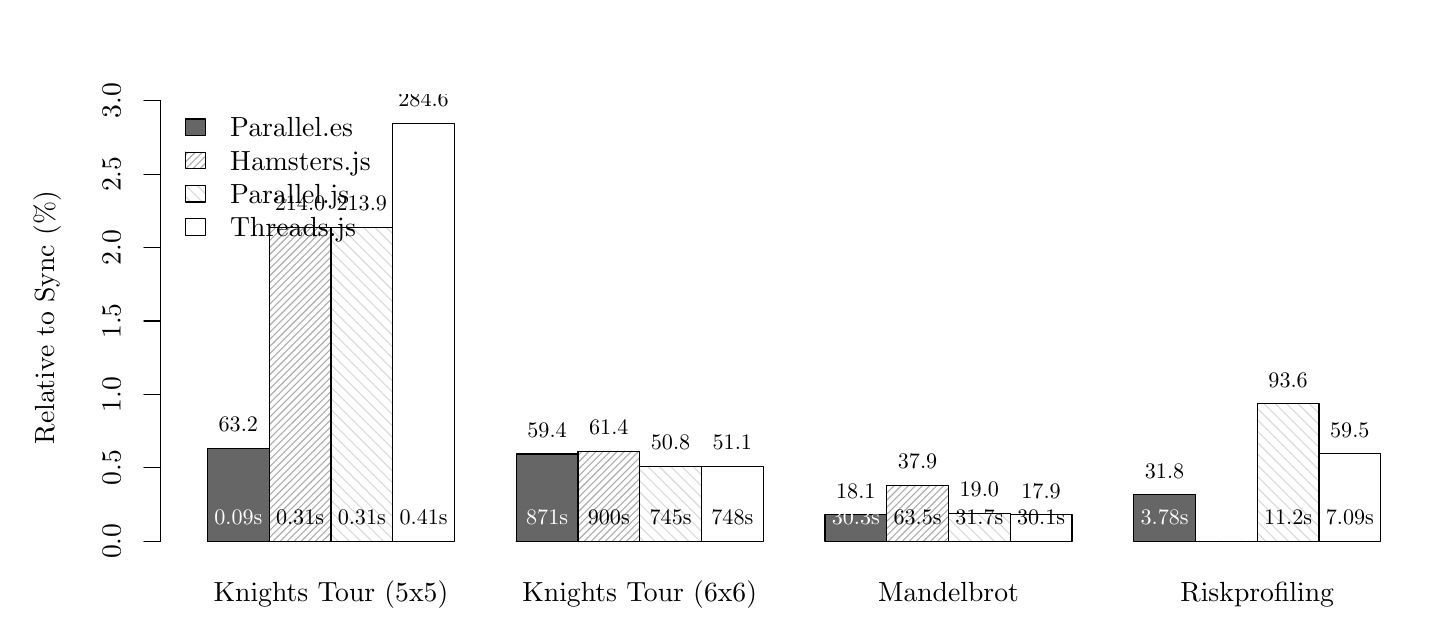
\begin{tikzpicture}[x=1pt,y=1pt]
\definecolor{fillColor}{RGB}{255,255,255}
\path[use as bounding box,fill=fillColor,fill opacity=0.00] (0,0) rectangle (505.89,209.58);
\begin{scope}
\path[clip] (  0.00,  0.00) rectangle (505.89,209.58);
\definecolor{fillColor}{gray}{0.40}

\path[fill=fillColor] ( 64.96, 24.00) --
	( 87.27, 24.00) --
	( 87.27, 57.51) --
	( 64.96, 57.51) --
	cycle;
\definecolor{drawColor}{RGB}{172,172,172}

\path[draw=drawColor,line width= 0.4pt,line join=round,line cap=round] ( 87.27,135.06) -- ( 89.73,137.52);

\path[draw=drawColor,line width= 0.4pt,line join=round,line cap=round] ( 87.27,132.51) -- ( 92.28,137.52);

\path[draw=drawColor,line width= 0.4pt,line join=round,line cap=round] ( 87.27,129.95) -- ( 94.84,137.52);

\path[draw=drawColor,line width= 0.4pt,line join=round,line cap=round] ( 87.27,127.40) -- ( 97.39,137.52);

\path[draw=drawColor,line width= 0.4pt,line join=round,line cap=round] ( 87.27,124.84) -- ( 99.95,137.52);

\path[draw=drawColor,line width= 0.4pt,line join=round,line cap=round] ( 87.27,122.29) -- (102.50,137.52);

\path[draw=drawColor,line width= 0.4pt,line join=round,line cap=round] ( 87.27,119.73) -- (105.06,137.52);

\path[draw=drawColor,line width= 0.4pt,line join=round,line cap=round] ( 87.27,117.18) -- (107.61,137.52);

\path[draw=drawColor,line width= 0.4pt,line join=round,line cap=round] ( 87.27,114.62) -- (109.59,136.94);

\path[draw=drawColor,line width= 0.4pt,line join=round,line cap=round] ( 87.27,112.07) -- (109.59,134.38);

\path[draw=drawColor,line width= 0.4pt,line join=round,line cap=round] ( 87.27,109.51) -- (109.59,131.83);

\path[draw=drawColor,line width= 0.4pt,line join=round,line cap=round] ( 87.27,106.96) -- (109.59,129.27);

\path[draw=drawColor,line width= 0.4pt,line join=round,line cap=round] ( 87.27,104.40) -- (109.59,126.71);

\path[draw=drawColor,line width= 0.4pt,line join=round,line cap=round] ( 87.27,101.85) -- (109.59,124.16);

\path[draw=drawColor,line width= 0.4pt,line join=round,line cap=round] ( 87.27, 99.29) -- (109.59,121.60);

\path[draw=drawColor,line width= 0.4pt,line join=round,line cap=round] ( 87.27, 96.74) -- (109.59,119.05);

\path[draw=drawColor,line width= 0.4pt,line join=round,line cap=round] ( 87.27, 94.18) -- (109.59,116.49);

\path[draw=drawColor,line width= 0.4pt,line join=round,line cap=round] ( 87.27, 91.62) -- (109.59,113.94);

\path[draw=drawColor,line width= 0.4pt,line join=round,line cap=round] ( 87.27, 89.07) -- (109.59,111.38);

\path[draw=drawColor,line width= 0.4pt,line join=round,line cap=round] ( 87.27, 86.51) -- (109.59,108.83);

\path[draw=drawColor,line width= 0.4pt,line join=round,line cap=round] ( 87.27, 83.96) -- (109.59,106.27);

\path[draw=drawColor,line width= 0.4pt,line join=round,line cap=round] ( 87.27, 81.40) -- (109.59,103.72);

\path[draw=drawColor,line width= 0.4pt,line join=round,line cap=round] ( 87.27, 78.85) -- (109.59,101.16);

\path[draw=drawColor,line width= 0.4pt,line join=round,line cap=round] ( 87.27, 76.29) -- (109.59, 98.61);

\path[draw=drawColor,line width= 0.4pt,line join=round,line cap=round] ( 87.27, 73.74) -- (109.59, 96.05);

\path[draw=drawColor,line width= 0.4pt,line join=round,line cap=round] ( 87.27, 71.18) -- (109.59, 93.50);

\path[draw=drawColor,line width= 0.4pt,line join=round,line cap=round] ( 87.27, 68.63) -- (109.59, 90.94);

\path[draw=drawColor,line width= 0.4pt,line join=round,line cap=round] ( 87.27, 66.07) -- (109.59, 88.39);

\path[draw=drawColor,line width= 0.4pt,line join=round,line cap=round] ( 87.27, 63.52) -- (109.59, 85.83);

\path[draw=drawColor,line width= 0.4pt,line join=round,line cap=round] ( 87.27, 60.96) -- (109.59, 83.28);

\path[draw=drawColor,line width= 0.4pt,line join=round,line cap=round] ( 87.27, 58.41) -- (109.59, 80.72);

\path[draw=drawColor,line width= 0.4pt,line join=round,line cap=round] ( 87.27, 55.85) -- (109.59, 78.17);

\path[draw=drawColor,line width= 0.4pt,line join=round,line cap=round] ( 87.27, 53.30) -- (109.59, 75.61);

\path[draw=drawColor,line width= 0.4pt,line join=round,line cap=round] ( 87.27, 50.74) -- (109.59, 73.06);

\path[draw=drawColor,line width= 0.4pt,line join=round,line cap=round] ( 87.27, 48.19) -- (109.59, 70.50);

\path[draw=drawColor,line width= 0.4pt,line join=round,line cap=round] ( 87.27, 45.63) -- (109.59, 67.95);

\path[draw=drawColor,line width= 0.4pt,line join=round,line cap=round] ( 87.27, 43.08) -- (109.59, 65.39);

\path[draw=drawColor,line width= 0.4pt,line join=round,line cap=round] ( 87.27, 40.52) -- (109.59, 62.84);

\path[draw=drawColor,line width= 0.4pt,line join=round,line cap=round] ( 87.27, 37.97) -- (109.59, 60.28);

\path[draw=drawColor,line width= 0.4pt,line join=round,line cap=round] ( 87.27, 35.41) -- (109.59, 57.73);

\path[draw=drawColor,line width= 0.4pt,line join=round,line cap=round] ( 87.27, 32.86) -- (109.59, 55.17);

\path[draw=drawColor,line width= 0.4pt,line join=round,line cap=round] ( 87.27, 30.30) -- (109.59, 52.62);

\path[draw=drawColor,line width= 0.4pt,line join=round,line cap=round] ( 87.27, 27.75) -- (109.59, 50.06);

\path[draw=drawColor,line width= 0.4pt,line join=round,line cap=round] ( 87.27, 25.19) -- (109.59, 47.51);

\path[draw=drawColor,line width= 0.4pt,line join=round,line cap=round] ( 88.64, 24.00) -- (109.59, 44.95);

\path[draw=drawColor,line width= 0.4pt,line join=round,line cap=round] ( 91.19, 24.00) -- (109.59, 42.40);

\path[draw=drawColor,line width= 0.4pt,line join=round,line cap=round] ( 93.75, 24.00) -- (109.59, 39.84);

\path[draw=drawColor,line width= 0.4pt,line join=round,line cap=round] ( 96.30, 24.00) -- (109.59, 37.29);

\path[draw=drawColor,line width= 0.4pt,line join=round,line cap=round] ( 98.86, 24.00) -- (109.59, 34.73);

\path[draw=drawColor,line width= 0.4pt,line join=round,line cap=round] (101.41, 24.00) -- (109.59, 32.17);

\path[draw=drawColor,line width= 0.4pt,line join=round,line cap=round] (103.97, 24.00) -- (109.59, 29.62);

\path[draw=drawColor,line width= 0.4pt,line join=round,line cap=round] (106.52, 24.00) -- (109.59, 27.06);

\path[draw=drawColor,line width= 0.4pt,line join=round,line cap=round] (109.08, 24.00) -- (109.59, 24.51);
\definecolor{drawColor}{RGB}{218,218,218}

\path[draw=drawColor,line width= 0.4pt,line join=round,line cap=round] (112.14, 24.00) -- (109.59, 26.56);

\path[draw=drawColor,line width= 0.4pt,line join=round,line cap=round] (116.23, 24.00) -- (109.59, 30.64);

\path[draw=drawColor,line width= 0.4pt,line join=round,line cap=round] (120.32, 24.00) -- (109.59, 34.73);

\path[draw=drawColor,line width= 0.4pt,line join=round,line cap=round] (124.41, 24.00) -- (109.59, 38.82);

\path[draw=drawColor,line width= 0.4pt,line join=round,line cap=round] (128.50, 24.00) -- (109.59, 42.91);

\path[draw=drawColor,line width= 0.4pt,line join=round,line cap=round] (131.90, 24.68) -- (109.59, 47.00);

\path[draw=drawColor,line width= 0.4pt,line join=round,line cap=round] (131.90, 28.77) -- (109.59, 51.09);

\path[draw=drawColor,line width= 0.4pt,line join=round,line cap=round] (131.90, 32.86) -- (109.59, 55.17);

\path[draw=drawColor,line width= 0.4pt,line join=round,line cap=round] (131.90, 36.95) -- (109.59, 59.26);

\path[draw=drawColor,line width= 0.4pt,line join=round,line cap=round] (131.90, 41.04) -- (109.59, 63.35);

\path[draw=drawColor,line width= 0.4pt,line join=round,line cap=round] (131.90, 45.12) -- (109.59, 67.44);

\path[draw=drawColor,line width= 0.4pt,line join=round,line cap=round] (131.90, 49.21) -- (109.59, 71.53);

\path[draw=drawColor,line width= 0.4pt,line join=round,line cap=round] (131.90, 53.30) -- (109.59, 75.62);

\path[draw=drawColor,line width= 0.4pt,line join=round,line cap=round] (131.90, 57.39) -- (109.59, 79.70);

\path[draw=drawColor,line width= 0.4pt,line join=round,line cap=round] (131.90, 61.48) -- (109.59, 83.79);

\path[draw=drawColor,line width= 0.4pt,line join=round,line cap=round] (131.90, 65.57) -- (109.59, 87.88);

\path[draw=drawColor,line width= 0.4pt,line join=round,line cap=round] (131.90, 69.65) -- (109.59, 91.97);

\path[draw=drawColor,line width= 0.4pt,line join=round,line cap=round] (131.90, 73.74) -- (109.59, 96.06);

\path[draw=drawColor,line width= 0.4pt,line join=round,line cap=round] (131.90, 77.83) -- (109.59,100.14);

\path[draw=drawColor,line width= 0.4pt,line join=round,line cap=round] (131.90, 81.92) -- (109.59,104.23);

\path[draw=drawColor,line width= 0.4pt,line join=round,line cap=round] (131.90, 86.01) -- (109.59,108.32);

\path[draw=drawColor,line width= 0.4pt,line join=round,line cap=round] (131.90, 90.09) -- (109.59,112.41);

\path[draw=drawColor,line width= 0.4pt,line join=round,line cap=round] (131.90, 94.18) -- (109.59,116.50);

\path[draw=drawColor,line width= 0.4pt,line join=round,line cap=round] (131.90, 98.27) -- (109.59,120.59);

\path[draw=drawColor,line width= 0.4pt,line join=round,line cap=round] (131.90,102.36) -- (109.59,124.67);

\path[draw=drawColor,line width= 0.4pt,line join=round,line cap=round] (131.90,106.45) -- (109.59,128.76);

\path[draw=drawColor,line width= 0.4pt,line join=round,line cap=round] (131.90,110.54) -- (109.59,132.85);

\path[draw=drawColor,line width= 0.4pt,line join=round,line cap=round] (131.90,114.62) -- (109.59,136.94);

\path[draw=drawColor,line width= 0.4pt,line join=round,line cap=round] (131.90,118.71) -- (113.15,137.46);

\path[draw=drawColor,line width= 0.4pt,line join=round,line cap=round] (131.90,122.80) -- (117.24,137.46);

\path[draw=drawColor,line width= 0.4pt,line join=round,line cap=round] (131.90,126.89) -- (121.33,137.46);

\path[draw=drawColor,line width= 0.4pt,line join=round,line cap=round] (131.90,130.98) -- (125.41,137.46);

\path[draw=drawColor,line width= 0.4pt,line join=round,line cap=round] (131.90,135.06) -- (129.50,137.46);

\path[fill=fillColor] (176.53, 24.00) --
	(198.84, 24.00) --
	(198.84, 55.54) --
	(176.53, 55.54) --
	cycle;
\definecolor{drawColor}{RGB}{172,172,172}

\path[draw=drawColor,line width= 0.4pt,line join=round,line cap=round] (198.84, 55.00) -- (200.43, 56.58);

\path[draw=drawColor,line width= 0.4pt,line join=round,line cap=round] (198.84, 52.44) -- (202.98, 56.58);

\path[draw=drawColor,line width= 0.4pt,line join=round,line cap=round] (198.84, 49.89) -- (205.54, 56.58);

\path[draw=drawColor,line width= 0.4pt,line join=round,line cap=round] (198.84, 47.33) -- (208.09, 56.58);

\path[draw=drawColor,line width= 0.4pt,line join=round,line cap=round] (198.84, 44.78) -- (210.65, 56.58);

\path[draw=drawColor,line width= 0.4pt,line join=round,line cap=round] (198.84, 42.22) -- (213.20, 56.58);

\path[draw=drawColor,line width= 0.4pt,line join=round,line cap=round] (198.84, 39.67) -- (215.76, 56.58);

\path[draw=drawColor,line width= 0.4pt,line join=round,line cap=round] (198.84, 37.11) -- (218.31, 56.58);

\path[draw=drawColor,line width= 0.4pt,line join=round,line cap=round] (198.84, 34.56) -- (220.87, 56.58);

\path[draw=drawColor,line width= 0.4pt,line join=round,line cap=round] (198.84, 32.00) -- (221.16, 54.32);

\path[draw=drawColor,line width= 0.4pt,line join=round,line cap=round] (198.84, 29.45) -- (221.16, 51.76);

\path[draw=drawColor,line width= 0.4pt,line join=round,line cap=round] (198.84, 26.89) -- (221.16, 49.21);

\path[draw=drawColor,line width= 0.4pt,line join=round,line cap=round] (198.84, 24.34) -- (221.16, 46.65);

\path[draw=drawColor,line width= 0.4pt,line join=round,line cap=round] (201.06, 24.00) -- (221.16, 44.10);

\path[draw=drawColor,line width= 0.4pt,line join=round,line cap=round] (203.62, 24.00) -- (221.16, 41.54);

\path[draw=drawColor,line width= 0.4pt,line join=round,line cap=round] (206.17, 24.00) -- (221.16, 38.99);

\path[draw=drawColor,line width= 0.4pt,line join=round,line cap=round] (208.73, 24.00) -- (221.16, 36.43);

\path[draw=drawColor,line width= 0.4pt,line join=round,line cap=round] (211.28, 24.00) -- (221.16, 33.88);

\path[draw=drawColor,line width= 0.4pt,line join=round,line cap=round] (213.84, 24.00) -- (221.16, 31.32);

\path[draw=drawColor,line width= 0.4pt,line join=round,line cap=round] (216.39, 24.00) -- (221.16, 28.77);

\path[draw=drawColor,line width= 0.4pt,line join=round,line cap=round] (218.95, 24.00) -- (221.16, 26.21);
\definecolor{drawColor}{RGB}{218,218,218}

\path[draw=drawColor,line width= 0.4pt,line join=round,line cap=round] (222.53, 24.00) -- (221.16, 25.37);

\path[draw=drawColor,line width= 0.4pt,line join=round,line cap=round] (226.61, 24.00) -- (221.16, 29.45);

\path[draw=drawColor,line width= 0.4pt,line join=round,line cap=round] (230.70, 24.00) -- (221.16, 33.54);

\path[draw=drawColor,line width= 0.4pt,line join=round,line cap=round] (234.79, 24.00) -- (221.16, 37.63);

\path[draw=drawColor,line width= 0.4pt,line join=round,line cap=round] (238.88, 24.00) -- (221.16, 41.72);

\path[draw=drawColor,line width= 0.4pt,line join=round,line cap=round] (242.97, 24.00) -- (221.16, 45.81);

\path[draw=drawColor,line width= 0.4pt,line join=round,line cap=round] (243.47, 27.58) -- (221.16, 49.90);

\path[draw=drawColor,line width= 0.4pt,line join=round,line cap=round] (243.47, 31.67) -- (224.16, 50.98);

\path[draw=drawColor,line width= 0.4pt,line join=round,line cap=round] (243.47, 35.76) -- (228.25, 50.98);

\path[draw=drawColor,line width= 0.4pt,line join=round,line cap=round] (243.47, 39.85) -- (232.34, 50.98);

\path[draw=drawColor,line width= 0.4pt,line join=round,line cap=round] (243.47, 43.93) -- (236.43, 50.98);

\path[draw=drawColor,line width= 0.4pt,line join=round,line cap=round] (243.47, 48.02) -- (240.52, 50.98);

\path[fill=fillColor] (288.10, 24.00) --
	(310.42, 24.00) --
	(310.42, 33.59) --
	(288.10, 33.59) --
	cycle;
\definecolor{drawColor}{RGB}{172,172,172}

\path[draw=drawColor,line width= 0.4pt,line join=round,line cap=round] (310.42, 43.92) -- (310.61, 44.12);

\path[draw=drawColor,line width= 0.4pt,line join=round,line cap=round] (310.42, 41.37) -- (313.16, 44.12);

\path[draw=drawColor,line width= 0.4pt,line join=round,line cap=round] (310.42, 38.81) -- (315.72, 44.12);

\path[draw=drawColor,line width= 0.4pt,line join=round,line cap=round] (310.42, 36.26) -- (318.27, 44.12);

\path[draw=drawColor,line width= 0.4pt,line join=round,line cap=round] (310.42, 33.70) -- (320.83, 44.12);

\path[draw=drawColor,line width= 0.4pt,line join=round,line cap=round] (310.42, 31.15) -- (323.38, 44.12);

\path[draw=drawColor,line width= 0.4pt,line join=round,line cap=round] (310.42, 28.59) -- (325.94, 44.12);

\path[draw=drawColor,line width= 0.4pt,line join=round,line cap=round] (310.42, 26.04) -- (328.49, 44.12);

\path[draw=drawColor,line width= 0.4pt,line join=round,line cap=round] (310.93, 24.00) -- (331.05, 44.12);

\path[draw=drawColor,line width= 0.4pt,line join=round,line cap=round] (313.49, 24.00) -- (332.73, 43.24);

\path[draw=drawColor,line width= 0.4pt,line join=round,line cap=round] (316.04, 24.00) -- (332.73, 40.69);

\path[draw=drawColor,line width= 0.4pt,line join=round,line cap=round] (318.60, 24.00) -- (332.73, 38.13);

\path[draw=drawColor,line width= 0.4pt,line join=round,line cap=round] (321.15, 24.00) -- (332.73, 35.58);

\path[draw=drawColor,line width= 0.4pt,line join=round,line cap=round] (323.71, 24.00) -- (332.73, 33.02);

\path[draw=drawColor,line width= 0.4pt,line join=round,line cap=round] (326.26, 24.00) -- (332.73, 30.47);

\path[draw=drawColor,line width= 0.4pt,line join=round,line cap=round] (328.82, 24.00) -- (332.73, 27.91);

\path[draw=drawColor,line width= 0.4pt,line join=round,line cap=round] (331.37, 24.00) -- (332.73, 25.36);
\definecolor{drawColor}{RGB}{218,218,218}

\path[draw=drawColor,line width= 0.4pt,line join=round,line cap=round] (332.91, 24.00) -- (332.73, 24.18);

\path[draw=drawColor,line width= 0.4pt,line join=round,line cap=round] (337.00, 24.00) -- (332.73, 28.26);

\path[draw=drawColor,line width= 0.4pt,line join=round,line cap=round] (341.08, 24.00) -- (332.73, 32.35);

\path[draw=drawColor,line width= 0.4pt,line join=round,line cap=round] (345.17, 24.00) -- (335.12, 34.06);

\path[draw=drawColor,line width= 0.4pt,line join=round,line cap=round] (349.26, 24.00) -- (339.20, 34.06);

\path[draw=drawColor,line width= 0.4pt,line join=round,line cap=round] (353.35, 24.00) -- (343.29, 34.06);

\path[draw=drawColor,line width= 0.4pt,line join=round,line cap=round] (355.05, 26.39) -- (347.38, 34.06);

\path[draw=drawColor,line width= 0.4pt,line join=round,line cap=round] (355.05, 30.48) -- (351.47, 34.06);

\path[fill=fillColor] (399.67, 24.00) --
	(421.99, 24.00) --
	(421.99, 40.85) --
	(399.67, 40.85) --
	cycle;
\definecolor{drawColor}{RGB}{172,172,172}

\path[draw=drawColor,line width= 0.4pt,line join=round,line cap=round] (423.36, 24.00) -- (423.36, 24.00);

\path[draw=drawColor,line width= 0.4pt,line join=round,line cap=round] (425.91, 24.00) -- (425.91, 24.00);

\path[draw=drawColor,line width= 0.4pt,line join=round,line cap=round] (428.47, 24.00) -- (428.47, 24.00);

\path[draw=drawColor,line width= 0.4pt,line join=round,line cap=round] (431.02, 24.00) -- (431.02, 24.00);

\path[draw=drawColor,line width= 0.4pt,line join=round,line cap=round] (433.58, 24.00) -- (433.58, 24.00);

\path[draw=drawColor,line width= 0.4pt,line join=round,line cap=round] (436.13, 24.00) -- (436.13, 24.00);

\path[draw=drawColor,line width= 0.4pt,line join=round,line cap=round] (438.69, 24.00) -- (438.69, 24.00);

\path[draw=drawColor,line width= 0.4pt,line join=round,line cap=round] (441.24, 24.00) -- (441.24, 24.00);

\path[draw=drawColor,line width= 0.4pt,line join=round,line cap=round] (443.80, 24.00) -- (443.80, 24.00);
\definecolor{drawColor}{RGB}{218,218,218}

\path[draw=drawColor,line width= 0.4pt,line join=round,line cap=round] (447.38, 24.00) -- (444.30, 27.07);

\path[draw=drawColor,line width= 0.4pt,line join=round,line cap=round] (451.47, 24.00) -- (444.30, 31.16);

\path[draw=drawColor,line width= 0.4pt,line join=round,line cap=round] (455.55, 24.00) -- (444.30, 35.25);

\path[draw=drawColor,line width= 0.4pt,line join=round,line cap=round] (459.64, 24.00) -- (444.30, 39.34);

\path[draw=drawColor,line width= 0.4pt,line join=round,line cap=round] (463.73, 24.00) -- (444.30, 43.43);

\path[draw=drawColor,line width= 0.4pt,line join=round,line cap=round] (466.62, 25.20) -- (444.30, 47.52);

\path[draw=drawColor,line width= 0.4pt,line join=round,line cap=round] (466.62, 29.29) -- (444.30, 51.60);

\path[draw=drawColor,line width= 0.4pt,line join=round,line cap=round] (466.62, 33.38) -- (444.30, 55.69);

\path[draw=drawColor,line width= 0.4pt,line join=round,line cap=round] (466.62, 37.47) -- (444.30, 59.78);

\path[draw=drawColor,line width= 0.4pt,line join=round,line cap=round] (466.62, 41.55) -- (444.30, 63.87);

\path[draw=drawColor,line width= 0.4pt,line join=round,line cap=round] (466.62, 45.64) -- (444.30, 67.96);

\path[draw=drawColor,line width= 0.4pt,line join=round,line cap=round] (466.62, 49.73) -- (444.30, 72.05);

\path[draw=drawColor,line width= 0.4pt,line join=round,line cap=round] (466.62, 53.82) -- (446.76, 73.68);

\path[draw=drawColor,line width= 0.4pt,line join=round,line cap=round] (466.62, 57.91) -- (450.84, 73.68);

\path[draw=drawColor,line width= 0.4pt,line join=round,line cap=round] (466.62, 62.00) -- (454.93, 73.68);

\path[draw=drawColor,line width= 0.4pt,line join=round,line cap=round] (466.62, 66.08) -- (459.02, 73.68);

\path[draw=drawColor,line width= 0.4pt,line join=round,line cap=round] (466.62, 70.17) -- (463.11, 73.68);
\definecolor{drawColor}{RGB}{0,0,0}

\path[draw=drawColor,line width= 0.4pt,line join=round,line cap=round] ( 64.96, 24.00) --
	( 87.27, 24.00) --
	( 87.27, 57.51) --
	( 64.96, 57.51) --
	( 64.96, 24.00);

\path[draw=drawColor,line width= 0.4pt,line join=round,line cap=round] ( 87.27, 24.00) --
	(109.59, 24.00) --
	(109.59,137.52) --
	( 87.27,137.52) --
	( 87.27, 24.00);

\path[draw=drawColor,line width= 0.4pt,line join=round,line cap=round] (109.59, 24.00) --
	(131.90, 24.00) --
	(131.90,137.46) --
	(109.59,137.46) --
	(109.59, 24.00);

\path[draw=drawColor,line width= 0.4pt,line join=round,line cap=round] (131.90, 24.00) --
	(154.22, 24.00) --
	(154.22,174.97) --
	(131.90,174.97) --
	(131.90, 24.00);

\path[draw=drawColor,line width= 0.4pt,line join=round,line cap=round] (176.53, 24.00) --
	(198.84, 24.00) --
	(198.84, 55.54) --
	(176.53, 55.54) --
	(176.53, 24.00);

\path[draw=drawColor,line width= 0.4pt,line join=round,line cap=round] (198.84, 24.00) --
	(221.16, 24.00) --
	(221.16, 56.58) --
	(198.84, 56.58) --
	(198.84, 24.00);

\path[draw=drawColor,line width= 0.4pt,line join=round,line cap=round] (221.16, 24.00) --
	(243.47, 24.00) --
	(243.47, 50.98) --
	(221.16, 50.98) --
	(221.16, 24.00);

\path[draw=drawColor,line width= 0.4pt,line join=round,line cap=round] (243.47, 24.00) --
	(265.79, 24.00) --
	(265.79, 51.09) --
	(243.47, 51.09) --
	(243.47, 24.00);

\path[draw=drawColor,line width= 0.4pt,line join=round,line cap=round] (288.10, 24.00) --
	(310.42, 24.00) --
	(310.42, 33.59) --
	(288.10, 33.59) --
	(288.10, 24.00);

\path[draw=drawColor,line width= 0.4pt,line join=round,line cap=round] (310.42, 24.00) --
	(332.73, 24.00) --
	(332.73, 44.12) --
	(310.42, 44.12) --
	(310.42, 24.00);

\path[draw=drawColor,line width= 0.4pt,line join=round,line cap=round] (332.73, 24.00) --
	(355.05, 24.00) --
	(355.05, 34.06) --
	(332.73, 34.06) --
	(332.73, 24.00);

\path[draw=drawColor,line width= 0.4pt,line join=round,line cap=round] (355.05, 24.00) --
	(377.36, 24.00) --
	(377.36, 33.52) --
	(355.05, 33.52) --
	(355.05, 24.00);

\path[draw=drawColor,line width= 0.4pt,line join=round,line cap=round] (399.67, 24.00) --
	(421.99, 24.00) --
	(421.99, 40.85) --
	(399.67, 40.85) --
	(399.67, 24.00);

\path[draw=drawColor,line width= 0.4pt,line join=round,line cap=round] (421.99, 24.00) --
	(444.30, 24.00) --
	(421.99, 24.00);

\path[draw=drawColor,line width= 0.4pt,line join=round,line cap=round] (444.30, 24.00) --
	(466.62, 24.00) --
	(466.62, 73.68) --
	(444.30, 73.68) --
	(444.30, 24.00);

\path[draw=drawColor,line width= 0.4pt,line join=round,line cap=round] (466.62, 24.00) --
	(488.93, 24.00) --
	(488.93, 55.57) --
	(466.62, 55.57) --
	(466.62, 24.00);
\end{scope}
\begin{scope}
\path[clip] (  0.00,  0.00) rectangle (505.89,209.58);
\definecolor{drawColor}{RGB}{0,0,0}

\node[text=drawColor,anchor=base,inner sep=0pt, outer sep=0pt, scale=  1.00] at (109.59,  2.40) {Knights Tour (5x5)};

\node[text=drawColor,anchor=base,inner sep=0pt, outer sep=0pt, scale=  1.00] at (221.16,  2.40) {Knights Tour (6x6)};

\node[text=drawColor,anchor=base,inner sep=0pt, outer sep=0pt, scale=  1.00] at (332.73,  2.40) {Mandelbrot};

\node[text=drawColor,anchor=base,inner sep=0pt, outer sep=0pt, scale=  1.00] at (444.30,  2.40) {Riskprofiling};
\end{scope}
\begin{scope}
\path[clip] (  0.00,  0.00) rectangle (505.89,209.58);
\definecolor{drawColor}{RGB}{0,0,0}

\node[text=drawColor,rotate= 90.00,anchor=base,inner sep=0pt, outer sep=0pt, scale=  1.00] at (  9.60,104.79) {Relative to Sync ({\%})};
\end{scope}
\begin{scope}
\path[clip] (  0.00,  0.00) rectangle (505.89,209.58);
\definecolor{drawColor}{RGB}{0,0,0}

\path[draw=drawColor,line width= 0.4pt,line join=round,line cap=round] ( 48.00, 24.00) -- ( 48.00,183.17);

\path[draw=drawColor,line width= 0.4pt,line join=round,line cap=round] ( 48.00, 24.00) -- ( 42.00, 24.00);

\path[draw=drawColor,line width= 0.4pt,line join=round,line cap=round] ( 48.00, 50.53) -- ( 42.00, 50.53);

\path[draw=drawColor,line width= 0.4pt,line join=round,line cap=round] ( 48.00, 77.06) -- ( 42.00, 77.06);

\path[draw=drawColor,line width= 0.4pt,line join=round,line cap=round] ( 48.00,103.58) -- ( 42.00,103.58);

\path[draw=drawColor,line width= 0.4pt,line join=round,line cap=round] ( 48.00,130.11) -- ( 42.00,130.11);

\path[draw=drawColor,line width= 0.4pt,line join=round,line cap=round] ( 48.00,156.64) -- ( 42.00,156.64);

\path[draw=drawColor,line width= 0.4pt,line join=round,line cap=round] ( 48.00,183.17) -- ( 42.00,183.17);

\node[text=drawColor,rotate= 90.00,anchor=base,inner sep=0pt, outer sep=0pt, scale=  1.00] at ( 33.60, 24.00) {0.0};

\node[text=drawColor,rotate= 90.00,anchor=base,inner sep=0pt, outer sep=0pt, scale=  1.00] at ( 33.60, 50.53) {0.5};

\node[text=drawColor,rotate= 90.00,anchor=base,inner sep=0pt, outer sep=0pt, scale=  1.00] at ( 33.60, 77.06) {1.0};

\node[text=drawColor,rotate= 90.00,anchor=base,inner sep=0pt, outer sep=0pt, scale=  1.00] at ( 33.60,103.58) {1.5};

\node[text=drawColor,rotate= 90.00,anchor=base,inner sep=0pt, outer sep=0pt, scale=  1.00] at ( 33.60,130.11) {2.0};

\node[text=drawColor,rotate= 90.00,anchor=base,inner sep=0pt, outer sep=0pt, scale=  1.00] at ( 33.60,156.64) {2.5};

\node[text=drawColor,rotate= 90.00,anchor=base,inner sep=0pt, outer sep=0pt, scale=  1.00] at ( 33.60,183.17) {3.0};
\end{scope}
\begin{scope}
\path[clip] ( 48.00, 24.00) rectangle (505.89,185.58);
\definecolor{fillColor}{gray}{0.40}

\path[fill=fillColor] ( 57.00,176.58) --
	( 64.20,176.58) --
	( 64.20,170.58) --
	( 57.00,170.58) --
	cycle;
\definecolor{drawColor}{RGB}{172,172,172}

\path[draw=drawColor,line width= 0.4pt,line join=round,line cap=round] ( 57.00,163.56) -- ( 58.03,164.58);

\path[draw=drawColor,line width= 0.4pt,line join=round,line cap=round] ( 57.00,161.00) -- ( 60.58,164.58);

\path[draw=drawColor,line width= 0.4pt,line join=round,line cap=round] ( 57.14,158.58) -- ( 63.14,164.58);

\path[draw=drawColor,line width= 0.4pt,line join=round,line cap=round] ( 59.69,158.58) -- ( 64.20,163.09);

\path[draw=drawColor,line width= 0.4pt,line join=round,line cap=round] ( 62.25,158.58) -- ( 64.20,160.54);
\definecolor{drawColor}{RGB}{218,218,218}

\path[draw=drawColor,line width= 0.4pt,line join=round,line cap=round] ( 59.06,146.58) -- ( 57.00,148.64);

\path[draw=drawColor,line width= 0.4pt,line join=round,line cap=round] ( 63.15,146.58) -- ( 57.15,152.58);

\path[draw=drawColor,line width= 0.4pt,line join=round,line cap=round] ( 64.20,149.62) -- ( 61.24,152.58);
\definecolor{drawColor}{RGB}{0,0,0}

\path[draw=drawColor,line width= 0.4pt,line join=round,line cap=round] ( 57.00,176.58) --
	( 64.20,176.58) --
	( 64.20,170.58) --
	( 57.00,170.58) --
	( 57.00,176.58);

\path[draw=drawColor,line width= 0.4pt,line join=round,line cap=round] ( 57.00,164.58) --
	( 64.20,164.58) --
	( 64.20,158.58) --
	( 57.00,158.58) --
	( 57.00,164.58);

\path[draw=drawColor,line width= 0.4pt,line join=round,line cap=round] ( 57.00,152.58) --
	( 64.20,152.58) --
	( 64.20,146.58) --
	( 57.00,146.58) --
	( 57.00,152.58);

\path[draw=drawColor,line width= 0.4pt,line join=round,line cap=round] ( 57.00,140.58) --
	( 64.20,140.58) --
	( 64.20,134.58) --
	( 57.00,134.58) --
	( 57.00,140.58);

\node[text=drawColor,anchor=base west,inner sep=0pt, outer sep=0pt, scale=  1.00] at ( 73.20,170.14) {Parallel.es};

\node[text=drawColor,anchor=base west,inner sep=0pt, outer sep=0pt, scale=  1.00] at ( 73.20,158.14) {Hamsters.js};

\node[text=drawColor,anchor=base west,inner sep=0pt, outer sep=0pt, scale=  1.00] at ( 73.20,146.14) {Parallel.js};

\node[text=drawColor,anchor=base west,inner sep=0pt, outer sep=0pt, scale=  1.00] at ( 73.20,134.14) {Threads.js};

\node[text=drawColor,anchor=base,inner sep=0pt, outer sep=0pt, scale=  0.80] at ( 76.12, 63.51) {63.2};

\node[text=drawColor,anchor=base,inner sep=0pt, outer sep=0pt, scale=  0.80] at ( 98.43,143.52) {214.0};

\node[text=drawColor,anchor=base,inner sep=0pt, outer sep=0pt, scale=  0.80] at (120.74,143.46) {213.9};

\node[text=drawColor,anchor=base,inner sep=0pt, outer sep=0pt, scale=  0.80] at (143.06,180.97) {284.6};

\node[text=drawColor,anchor=base,inner sep=0pt, outer sep=0pt, scale=  0.80] at (187.69, 61.54) {59.4};

\node[text=drawColor,anchor=base,inner sep=0pt, outer sep=0pt, scale=  0.80] at (210.00, 62.58) {61.4};

\node[text=drawColor,anchor=base,inner sep=0pt, outer sep=0pt, scale=  0.80] at (232.32, 56.98) {50.8};

\node[text=drawColor,anchor=base,inner sep=0pt, outer sep=0pt, scale=  0.80] at (254.63, 57.09) {51.1};

\node[text=drawColor,anchor=base,inner sep=0pt, outer sep=0pt, scale=  0.80] at (299.26, 39.59) {18.1};

\node[text=drawColor,anchor=base,inner sep=0pt, outer sep=0pt, scale=  0.80] at (321.57, 50.12) {37.9};

\node[text=drawColor,anchor=base,inner sep=0pt, outer sep=0pt, scale=  0.80] at (343.89, 40.06) {19.0};

\node[text=drawColor,anchor=base,inner sep=0pt, outer sep=0pt, scale=  0.80] at (366.20, 39.52) {17.9};

\node[text=drawColor,anchor=base,inner sep=0pt, outer sep=0pt, scale=  0.80] at (410.83, 46.85) {31.8};

\node[text=drawColor,anchor=base,inner sep=0pt, outer sep=0pt, scale=  0.80] at (455.46, 79.68) {93.6};

\node[text=drawColor,anchor=base,inner sep=0pt, outer sep=0pt, scale=  0.80] at (477.77, 61.57) {59.5};
\definecolor{drawColor}{RGB}{255,255,255}

\node[text=drawColor,anchor=base,inner sep=0pt, outer sep=0pt, scale=  0.80] at ( 76.12, 30.00) {0.09s};
\definecolor{drawColor}{RGB}{0,0,0}

\node[text=drawColor,anchor=base,inner sep=0pt, outer sep=0pt, scale=  0.80] at ( 98.43, 30.00) {0.31s};

\node[text=drawColor,anchor=base,inner sep=0pt, outer sep=0pt, scale=  0.80] at (120.74, 30.00) {0.31s};

\node[text=drawColor,anchor=base,inner sep=0pt, outer sep=0pt, scale=  0.80] at (143.06, 30.00) {0.41s};
\definecolor{drawColor}{RGB}{255,255,255}

\node[text=drawColor,anchor=base,inner sep=0pt, outer sep=0pt, scale=  0.80] at (187.69, 30.00) {871s};
\definecolor{drawColor}{RGB}{0,0,0}

\node[text=drawColor,anchor=base,inner sep=0pt, outer sep=0pt, scale=  0.80] at (210.00, 30.00) {900s};

\node[text=drawColor,anchor=base,inner sep=0pt, outer sep=0pt, scale=  0.80] at (232.32, 30.00) {745s};

\node[text=drawColor,anchor=base,inner sep=0pt, outer sep=0pt, scale=  0.80] at (254.63, 30.00) {748s};
\definecolor{drawColor}{RGB}{255,255,255}

\node[text=drawColor,anchor=base,inner sep=0pt, outer sep=0pt, scale=  0.80] at (299.26, 30.00) {30.3s};
\definecolor{drawColor}{RGB}{0,0,0}

\node[text=drawColor,anchor=base,inner sep=0pt, outer sep=0pt, scale=  0.80] at (321.57, 30.00) {63.5s};

\node[text=drawColor,anchor=base,inner sep=0pt, outer sep=0pt, scale=  0.80] at (343.89, 30.00) {31.7s};

\node[text=drawColor,anchor=base,inner sep=0pt, outer sep=0pt, scale=  0.80] at (366.20, 30.00) {30.1s};
\definecolor{drawColor}{RGB}{255,255,255}

\node[text=drawColor,anchor=base,inner sep=0pt, outer sep=0pt, scale=  0.80] at (410.83, 30.00) {3.78s};
\definecolor{drawColor}{RGB}{0,0,0}

\node[text=drawColor,anchor=base,inner sep=0pt, outer sep=0pt, scale=  0.80] at (455.46, 30.00) {11.2s};

\node[text=drawColor,anchor=base,inner sep=0pt, outer sep=0pt, scale=  0.80] at (477.77, 30.00) {7.09s};
\end{scope}
\end{tikzpicture}
